% !TeX program = pdflatex
% Academic CV of Angelo Rodio.
% Build: latexmk -pdf cv_academic.tex   (the PDF served on the website is assets/pdf/cv.pdf)

\documentclass[10pt,a4paper]{article}

% -------------------- Fonts and typography --------------------
\usepackage[T1]{fontenc}
\usepackage[utf8]{inputenc}
\usepackage[english]{babel}
\usepackage{XCharter}
\usepackage[scaled=0.92]{sourcesanspro}
\usepackage{microtype}
\usepackage{fontawesome5}

% -------------------- Layout --------------------
\usepackage[a4paper,top=1.7cm,bottom=1.8cm,left=1.9cm,right=1.9cm]{geometry}
\usepackage{xcolor}
\usepackage{graphicx}
\usepackage{tabularx}
\usepackage{enumitem}
\usepackage{titlesec}
\usepackage{fancyhdr}
\usepackage{lastpage}
\usepackage[hidelinks]{hyperref}
\usepackage{xurl}
\usepackage{etoolbox}
\urlstyle{same}
\usepackage{needspace}
\usepackage{array}

\definecolor{accent}{HTML}{1F4E79}
\definecolor{muted}{HTML}{555555}

\setlength{\parindent}{0pt}
\setlength{\parskip}{0pt}
\linespread{1.04}

\pagestyle{fancy}
\fancyhf{}
\renewcommand{\headrulewidth}{0pt}
\fancyfoot[L]{\small\color{muted}Angelo Rodio \textperiodcentered{} Curriculum Vitae}
\fancyfoot[R]{\small\color{muted}\thepage/\pageref{LastPage}}

\titleformat{\section}{\sffamily\large\bfseries\color{accent}}{}{0pt}{}[\vspace{-0.55em}\color{accent}\rule{\linewidth}{0.6pt}]
\titlespacing*{\section}{0pt}{1.0em}{0.55em}
\let\cvsection\section
\renewcommand{\section}[1]{\needspace{7\baselineskip}\cvsection{#1}}

\setlist[itemize]{leftmargin=1.1em,itemsep=0.12em,topsep=0.15em,parsep=0pt,label={\color{accent}\textbullet}}

% -------------------- Entry macros --------------------
% \entry{dates}{title}{institution and place}{details (may be empty)}
\newcommand{\entry}[4]{%
  \noindent\begin{tabularx}{\linewidth}{@{}>{\raggedright\arraybackslash}p{2.45cm}@{\hspace{0.35cm}}X@{}}
    \leavevmode\textcolor{muted}{\small #1} & \textbf{#2}\ifblank{#3}{}{, #3}\ifblank{#4}{}{\newline{\small #4}}
  \end{tabularx}\par\vspace{0.42em}}

% \item-like line with a date column
\newcommand{\dated}[2]{%
  \noindent\begin{tabularx}{\linewidth}{@{}>{\raggedright\arraybackslash}p{2.45cm}@{\hspace{0.35cm}}X@{}}
    \leavevmode\textcolor{muted}{\small #1} & #2
  \end{tabularx}\par\vspace{0.3em}}

\newcommand{\me}{\textbf{A.~Rodio}}
\newcommand{\venue}[1]{\textit{#1}}
\newcommand{\doi}[1]{\href{https://doi.org/#1}{\small\color{accent}\nolinkurl{doi:#1}}}
\newcommand{\arxiv}[1]{\href{https://arxiv.org/abs/#1}{\small\color{accent}arXiv:#1}}

% publication lists share one counter, so numbering runs [1], [2], ... across all blocks
\newcounter{pubno}
\newenvironment{publist}{%
  \begin{list}{\small\color{muted}[\arabic{pubno}]}{%
    \setlength{\leftmargin}{2.8em}\setlength{\labelwidth}{2.4em}\setlength{\labelsep}{0.4em}%
    \setlength{\itemsep}{0.28em}\setlength{\topsep}{0.1em}\setlength{\parsep}{0pt}}}%
  {\end{list}}
\newcommand{\pub}{\stepcounter{pubno}\item}

\begin{document}

% ==================== Header ====================
\begin{minipage}[t]{0.78\linewidth}
  \vspace{0pt}
  {\sffamily\fontsize{24}{28}\selectfont\bfseries\color{accent}Angelo Rodio}\\[0.35em]
  {\large Postdoctoral Researcher}\\[0.15em]
  Department of Electrical Engineering (ISY), Linköping University, Sweden\\[0.55em]
  {\small
  \faMapMarker*\ Campus Valla, B-huset, Entrance 29, Office 3A:469, 583\,30 Linköping, Sweden\\[0.12em]
  \faPhone*\ +46\,76\,447\,68\,29 \quad
  \faEnvelope[regular]\ \href{mailto:angelo.rodio@liu.se}{angelo.rodio@liu.se}, \href{mailto:a.rodio@yahoo.com}{a.rodio@yahoo.com}\\[0.12em]
  \faGlobe\ \href{https://arodio.github.io}{arodio.github.io} \quad
  \faGraduationCap\ \href{https://scholar.google.com/citations?user=l-uI1ioAAAAJ}{Google Scholar} \quad
  \faGithub\ \href{https://github.com/arodio}{arodio} \quad
  \faOrcid\ \href{https://orcid.org/0000-0001-8395-4536}{0000-0001-8395-4536}\\[0.12em]
  Italian \textperiodcentered{} born 6 July 1995 in Bari, Italy}
\end{minipage}\hfill
\begin{minipage}[t]{0.17\linewidth}
  \vspace{0pt}\raggedleft
  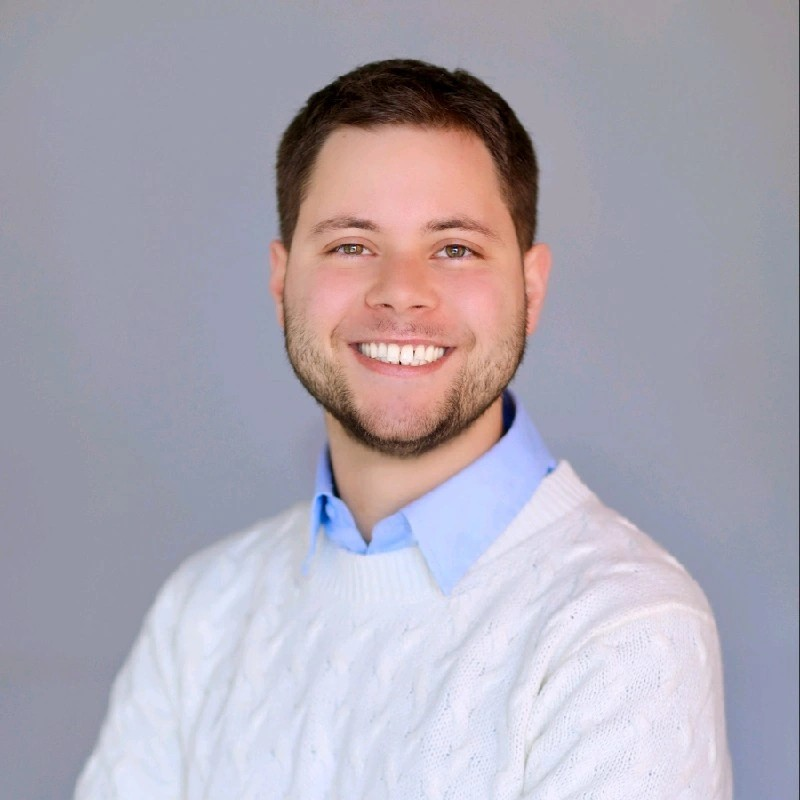
\includegraphics[width=\linewidth]{photo.jpeg}
\end{minipage}

% ==================== Research ====================
\section{Research interests}
Decentralized machine learning over networks: convergence theory, communication design, privacy, and energy efficiency.
Methods: convex and non-convex optimization, linear algebra, graph theory, stochastic modeling, and statistical learning theory.

% ==================== Qualifications ====================
\section{Academic qualifications}
\entry{Mar 2026}{Qualification aux fonctions de Maître de conférences}{France}
  {National qualification for associate professor positions, CNU Section 27 (Computer Science).}

% ==================== Positions ====================
\section{Positions}
\entry{Sep 2024 -- present}{Postdoctoral Researcher}{Linköping University, Sweden}
  {Division of Communication Systems. Hosts: Prof.\ Erik G.\ Larsson and Assoc.\ Prof.\ Zheng Chen.}
\entry{Jul -- Sep 2026}{Visiting Researcher}{Nanyang Technological University (NTU), Singapore}
  {College of Computing and Data Science. Host: Assoc.\ Prof.\ Chee Wei Tan. Funded by Vinnova (project MADELEINE, ref.\ 2026-01731, SEK\,500,000).}
\entry{Sep 2020 -- Mar 2021}{Telecommunications Engineer}{TIM S.p.A., Rome, Italy}
  {Consulting and integration support for a cloud platform.}

% ==================== Education ====================
\section{Education}
\entry{Apr 2021 -- Jul 2024}{PhD in Computer Science}{Inria and Université Côte d'Azur, France}
  {Thesis: \textit{Client Heterogeneity in Federated Learning Systems}, defended 3 July 2024.
   Supervisors: Giovanni Neglia and Alain Jean-Marie.
   Reviewers: H.\ Vincent Poor (Princeton University) and Michele Rossi (University of Padova).
   Funded by a 3IA Côte d'Azur doctoral fellowship.}
\entry{Sep 2019 -- Aug 2020}{MSc in Computer Engineering (double degree)}{Université Côte d'Azur, France}
  {Grade: \textit{Très bien}. Thesis at Inria on Wi-Fi fingerprint indoor localization for smartphones (supervisors: Arnaud Legout and Chadi Barakat).}
\entry{Oct 2018 -- Sep 2020}{MSc in Telecommunications Engineering}{Politecnico di Bari, Italy}
  {Grade: 110/110 \textit{cum laude}. Supervisor: Luigi Alfredo Grieco.}
\entry{Sep 2014 -- Feb 2018}{BSc in Computer Engineering}{Politecnico di Bari, Italy}
  {Grade: 109/110. Thesis on the performance of nanoscale communication systems (supervisors: Giuseppe Piro and Gennaro Boggia).}

% ==================== Grants ====================
\section{Grants and awards}
\dated{2026}{\textbf{Vinnova mobility grant}, SEK\,500,000, for the project MADELEINE: \textit{Massive Decentralised Learning in the Network Edge} (ref.\ 2026-01731).
  Call: \textit{Individual mobility within 6G for collaborations with the USA and Singapore}.
  Sole applicant and project leader. The grant funded a research stay at NTU Singapore and started a new collaboration between LiU and NTU.}
\dated{2025}{\textbf{IEEE Information Theory Society travel grant}, IEEE ITW 2025.}
\dated{2024}{\textbf{ACM SIGMETRICS student travel grant}, ACM SIGMETRICS 2024.}
\dated{2021}{\textbf{3IA Côte d'Azur doctoral fellowship} (PhD funding).}

% ==================== Publications ====================
\section{Publications}
{\small\color{muted}Google Scholar: \href{https://scholar.google.com/citations?user=l-uI1ioAAAAJ}{scholar.google.com/citations?user=l-uI1ioAAAAJ}. My name in bold.}

\vspace{0.4em}
\textbf{Journal articles}
\begin{publist}
  \pub D.\,R.~Arputharaj, C.~Rodriguez, \me, G.~Neglia.
    Carbon-Aware Client and Time Scheduling for Green Federated Learning.
    \venue{Performance Evaluation}, art.\ 102597, 2026. \doi{10.1016/j.peva.2026.102597}
  \pub C.~Xu, C.~Kaplan, \me, T.~Si~Salem, G.~Neglia.
    Federated Learning for Collaborative Inference Systems: The Case of Early Exit Networks.
    \venue{Performance Evaluation}, vol.\ 171, art.\ 102538, 2026. \doi{10.1016/j.peva.2025.102538}
  \pub \me, F.~Faticanti, O.~Marfoq, G.~Neglia, E.~Leonardi.
    Federated Learning Under Heterogeneous and Correlated Client Availability.
    \venue{IEEE/ACM Transactions on Networking}, 32(2):1451--1460, 2024. \doi{10.1109/TNET.2023.3324257}
\end{publist}

\textbf{Conference papers}
\begin{publist}
  \pub \me, G.~Neglia, Z.~Chen, E.\,G.~Larsson.
    A Unified Convergence Analysis for Semi-Decentralized Learning: Sampled-to-Sampled vs.\ Sampled-to-All Communication.
    \venue{AAAI Conference on Artificial Intelligence (AAAI)}, 2026. \textbf{Oral presentation.} \doi{10.1609/aaai.v40i30.39705}
  \pub D.~Pérez~Herrera, \me, Z.~Chen, E.\,G.~Larsson.
    Power Allocation for Average Consensus in Wireless Networks with Link Failures.
    \venue{European Wireless Conference (EW)}, pp.\ 172--177, 2025.
  \pub D.\,R.~Arputharaj, C.~Rodriguez, \me, G.~Neglia.
    Green Federated Learning via Carbon-Aware Client and Time Slot Scheduling.
    \venue{IEEE MASCOTS}, 2025. \doi{10.1109/MASCOTS67699.2025.11283314}
  \pub \me, Z.~Chen, E.\,G.~Larsson.
    Optimizing Privacy-Utility Trade-off in Decentralized Learning with Generalized Correlated Noise.
    \venue{IEEE Information Theory Workshop (ITW)}, 2025. \doi{10.1109/ITW62417.2025.11240322}
  \pub \me, G.~Neglia.
    FedStale: Leveraging Stale Updates in Federated Learning.
    \venue{European Conference on Artificial Intelligence (ECAI)}, pp.\ 3071--3078, 2024. \doi{10.3233/FAIA240849}
  \pub \me, G.~Neglia, F.~Busacca, S.~Mangione, S.~Palazzo, F.~Restuccia, I.~Tinnirello.
    Federated Learning with Packet Losses.
    \venue{International Symposium on Wireless Personal Multimedia Communications (WPMC)}, 2023. \doi{10.1109/WPMC59531.2023.10338845}
  \pub \me, F.~Faticanti, O.~Marfoq, G.~Neglia, E.~Leonardi.
    Federated Learning under Heterogeneous and Correlated Client Availability.
    \venue{IEEE INFOCOM}, 2023. \doi{10.1109/INFOCOM53939.2023.10228876}
  \pub \me.
    The Many Facets of Variance Reduction in Federated Learning.
    \venue{ACM SIGMETRICS Performance Evaluation Review} 52(4):11--12, 2025 (poster at ACM SIGMETRICS 2024). \doi{10.1145/3725536.3725542}
\end{publist}

\textbf{Under review}
\begin{publist}
  \pub D.~Pérez~Herrera, \me, Z.~Chen, E.\,G.~Larsson.
    Heterogeneity-Aware Topology and Mixing Matrix Design for Decentralized Learning.
    Submitted to \venue{IEEE Transactions on Signal and Information Processing over Networks}.
\end{publist}

\textbf{PhD thesis}
\begin{publist}
  \pub \me. Client Heterogeneity in Federated Learning Systems. PhD thesis, Université Côte d'Azur, 2024.
    \href{https://theses.hal.science/tel-04685040}{\small\color{accent}HAL: tel-04685040}
\end{publist}

% ==================== Teaching ====================
\section{Teaching}
{\small\color{muted}79 hours at Master's level, taught in English in Sweden and France.}\par\vspace{0.4em}
\entry{2026}{Distributed Information Processing and Machine Learning (TSKS38)}{Linköping University}
  {28 h: 12 h of tutorials and 16 h of labs (with A.~Edin).}
\entry{2025}{Distributed Information Processing and Machine Learning (TSKS38)}{Linköping University}
  {12 h of tutorials. Prepared the problems and solutions, and graded the exams.}
\entry{2022 -- 2024}{Federated Learning and Data Privacy}{Université Côte d'Azur (M2 DS4H)}
  {12 h of labs per year (2022--23 and 2023--24, including 3 h co-taught with C.~Xu).}
\entry{2021 -- 2022}{Optimization for Machine Learning}{Université Côte d'Azur (M1 DS4H)}
  {15 h of labs (including 9 h co-taught with O.~Marfoq).}

% ==================== Supervision ====================
\section{Supervision}
\dated{2026}{\textbf{Mehran Mamivand}, MSc thesis, Linköping University.
  \textit{Energy-Efficient Semi-Decentralized Federated Learning via Cooperative D2D Model Aggregation}.}
\dated{2026}{\textbf{Camilla Samuelsson}, MSc thesis, Linköping University, carried out at the Swedish Defence Research Agency (FOI).
  \textit{Set Reconciliation Algorithms in Tactical Networks}.}
\dated{2024}{\textbf{Albachiara Bellaroba}, MSc thesis, Sapienza University of Rome, Italy.}
\dated{2023}{\textbf{Mohamed Salah Jebali}, MSc thesis, University of Florence, Italy.}
\dated{2023}{\textbf{Maysae Hmamouchi}, MSc research project, Université Côte d'Azur, France.}

% ==================== Service ====================
\section{Service}
\dated{Session chair}{AAAI Conference on Artificial Intelligence (AAAI 2026); IEEE Information Theory Workshop (ITW 2025).}
\dated{Reviewer}{\textit{Journals:} IEEE Journal on Selected Areas in Communications; IEEE Transactions on Automatic Control; IEEE Transactions on Mobile Computing; Computer Networks.\newline
  \textit{Conferences:} AAAI, UAI, IEEE INFOCOM, IEEE GLOBECOM, IEEE ICC, IEEE ICASSP.}
\dated{Evaluation}{Evaluator of Master's final projects, MSc Data Science and Artificial Intelligence, Université Côte d'Azur, 2023.}

% ==================== Skills ====================
\section{Skills and languages}
\dated{Programming}{Python, C/C++, Java; Linux, Git, Jupyter notebooks; reproducible research code.}
\dated{Languages}{Italian (native), English (C1), French (B2).}

% ==================== References ====================
\section{References}
\begin{tabularx}{\linewidth}{@{}X@{\hspace{0.8cm}}X@{}}
  \textbf{Prof.\ Erik G.\ Larsson} &
  \textbf{Dr.\ Giovanni Neglia} \\
  {\small Professor and Head of the Division of Communication Systems, Linköping University, Sweden} &
  {\small Research Director, Inria, Head of the NEO team, 3IA Côte d'Azur Chair, France} \\
  {\small\href{mailto:erik.g.larsson@liu.se}{erik.g.larsson@liu.se} \textperiodcentered{} +46\,13\,28\,13\,12} &
  {\small\href{mailto:giovanni.neglia@inria.fr}{giovanni.neglia@inria.fr} \textperiodcentered{} +33\,4\,92\,38\,79\,06}
\end{tabularx}

\vfill
{\small\color{muted}Last updated: October 2026.}

\end{document}
